\scanpage{72}\mspage{71}

Pour la suite, il faut faire attention si les axiomes vont passer aux sous-contrées. Introduisons quand $= =$ la définition en forme

\uline{Définition 1} On appelle
% fig-pleine: the words occur once; the long hooked leader is distinct from their underlines.
\figure{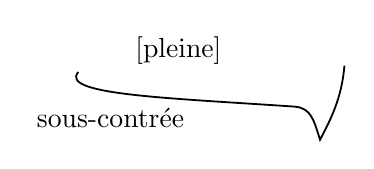
\begin{tikzpicture}[x=1cm,y=1cm]
\node[anchor=west] (s) at (0,0) {\uline{sous-contrée}};
\node[anchor=west] at (1.25,.85) {\inserted{[\uline{pleine}]}};
\draw[line width=.65pt] (.65,.58) .. controls (.4,.29) and (1.8,.25) .. (3.4,.14) .. controls (3.61,.12) and (3.64,-.03) .. (3.72,-.28) .. controls (3.92,.09) and (4.0,.33) .. (4.03,.66);
\end{tikzpicture}}
de la contrée $\unsure{\deleted{\mathcal F}\mathcal C|\mathscr C|\mathbb C}=(\mathcal F,\leq,\preceq)$, \unsure{tout|\deleted{tout}} sous-ens. qui \unsure{satisfait|satisfont} les conditions

a) fermé pour $\leq$, et stable par sup quelc. pour $\leq$ [et à ce titre, s'en correspond,
% fig-a-insertions: raised par phrase and M' with their separate connecting strokes.
\figure{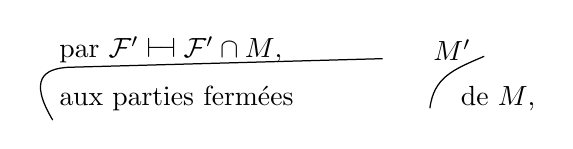
\begin{tikzpicture}[x=1cm,y=1cm]
\node[anchor=west] at (0,0) {aux parties fermées};
\node[anchor=west] at (5.1,0) {de $M$,};
\node[anchor=west] at (0,.62) {\inserted{par $\mathcal F'\mathrel{\vdash\joinrel\dashv}\mathcal F'\cap M$,}};
\node[anchor=west] at (4.75,.62) {\inserted{$M'$}};
\draw[line width=.45pt] (.04,-.27) .. controls (-.27,.25) and (-.07,.38) .. (.23,.4) -- (4.23,.51);
\draw[line width=.45pt] (4.83,-.12) .. controls (4.88,.27) and (5.12,.37) .. (5.52,.54);
\end{tikzpicture}}
par $M'\unsure{\mathrel{\mapstochar\relbar}|\mathrel{\vdash\joinrel\dashv}|\mapsto}\mathcal F'=\{F\in\mathcal F\mid\overline F\subset M'\}$].

% slanted
\margin{Je ne sais s'il faut prendre des sup quelconques \unsure{(condition stricte)|(condition stricts)} \deleted{\unsure{et}} ou bien \unsure{de|des} sup finis seulement \unsure{(condition large)|(condition lge)}}

b) fermé pour $\preceq$ (ce qui impose une restriction aux parties envisagées $M'$ de $M$\unsure{\}|?}, \deleted{\unsure{à savoir|savoir} : si $X\in$} \inserted{qu'on va formuler} plus bas)

% fig-marginal-c: right marginal continuation, including its descending hooked pointer.
% The dark initial before ous-fig. and the strokes below it occupy ONE worked position.
\figure{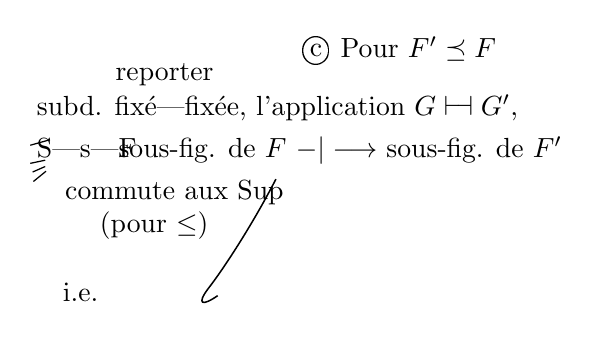
\begin{tikzpicture}[x=1cm,y=1cm]
\node[anchor=west] at (1.0,3.05) {reporter};
\node[anchor=west] at (3.35,3.35) {\textcircled{c} Pour $F'\preceq F$};
\node[anchor=west] at (0,2.62) {subd. \unsure{fixé|fixée}, l'application $G\mathrel{\vdash\joinrel\dashv}G'$,};
\node[anchor=west] at (0,2.08) {\unsure{S|s|\rlap{\deleted{F}}s}ous-fig. de $F$ $\unsure{-|\longrightarrow}$ sous-fig. de $F'$};
\draw[line width=.45pt] (.04,2.15) -- (.29,2.22);
\draw[line width=.45pt] (.04,1.92) -- (.23,1.96);
\draw[line width=.45pt] (.07,1.81) -- (.23,1.88);
\draw[line width=.45pt] (.08,1.69) -- (.24,1.82);
\node[anchor=west] at (.36,1.55) {commute aux Sup};
\node[anchor=west] at (.8,1.13) {(pour $\leq$)};
\node[anchor=west] at (.33,.28) {i.e.};
\draw[line width=.55pt] (3.16,1.72) .. controls (2.85,1.12) and (2.48,.56) .. (2.3,.33) .. controls (2.15,.13) and (2.22,.1) .. (2.42,.24);
\end{tikzpicture}}

% fig-C6-group: two literal diagrams, the oblique note, left rule, detached points,
% and the right note with its paired rules. Text is not duplicated outside this group.
\diagram{\begin{tikzpicture}[x=1cm,y=1cm]
\node[anchor=west] at (.4,0) {\uline{C6}};
\node[anchor=west] at (2.35,0) {Soit};
% diagram-C6-first
\node[anchor=north west] at (3.3,-.55) {\begin{tikzcd}[ampersand replacement=\&,column sep=1.4em,row sep=1em]
F' \arrow[r,phantom,"{\preceq}" description] \& F \arrow[d,phantom,"{\rotatebox{90}{$\leq$}}" description] \\
\& G
\end{tikzcd}};
\node[anchor=west] at (9.0,-1.02) {\unsure{de|dans|ds} $\mathcal F$};
% detached-points-C6: two separate marks, down-right arrangement, no assigned function.
\fill (2.25,-.84) circle (.022);
\fill (2.34,-.91) circle (.024);
% slanted, crossing the long rule
\node[anchor=west,align=left,rotate=43] at (-1.35,-1.98) {\unsure{symétrique|symetrique} en\\$\leq,\preceq$};
\draw[line width=.45pt] (.15,-.16) .. controls (.11,-1.5) and (.15,-2.7) .. (.18,-4.49) .. controls (.18,-4.7) and (.2,-4.81) .. (.25,-4.91);
\node[anchor=west] at (.35,-2.65) {\textcircled{a} Alors il existe un unique $H\in\mathcal F$ \unsure{avec|ou}};
% diagram-C6-square
\node[anchor=north west] at (3.45,-3.18) {\begin{tikzcd}[ampersand replacement=\&,column sep=1.4em,row sep=1em]
F' \arrow[r,phantom,"{\preceq}" description] \arrow[d,phantom,"{\rotatebox{90}{$\leq$}}" description] \& F \arrow[d,phantom,"{\rotatebox{90}{$\leq$}}" description] \\
G' \arrow[r,phantom,"{\preceq}" description] \& G
\end{tikzcd}};
% note-C6-b and paired rules
\node[anchor=north west,align=left] at (7.8,-2.93) {et \raisebox{.65ex}{\textcircled{b}} les \unsure{strates|str.tes} de\\
$G'$ sont les \deleted{\unsure{S}} \unsure{strates|str.tes}\\
$X'$ de $F'$ \unsure{tel|\deleted{tel}}les que\\
$X'\ll\unsure{G_m|G_n|G}$.\\
Ce compl\unsure{é|e}ment \unsure{servira}\\plus bas};
\draw[line width=.55pt] (7.62,-3.2) -- (7.67,-5.03);
\draw[line width=.55pt] (7.73,-3.19) -- (7.76,-5.05);
\draw[line width=.65pt] (7.63,-4.78) -- (7.78,-4.86);
\draw[line width=.55pt] (7.69,-4.67) -- (7.63,-5.02);
\end{tikzpicture}}

% slanted, at the lower left alongside the following paragraph
\margin{sur la sous-figure $G$ de $F$}
On dit que $G'$ est la \uline{subd} \uline{de} $G$ induite par la subd $F'$ de $\unsure{F|F'}$, ou que $G'$ est la \deleted{\unsure{sous-fig}}
